\section{Experiments}
\label{sec:experiments}

\subsection{Experimental Setup}
\label{sec:setup}

We evaluate our method on 11 triangle meshes spanning three orders of magnitude in vertex count: three small meshes (34K--50K vertices), five medium meshes (112K--544K), and three large meshes (1.2M--2.8M). The meshes are selected to cover a range of geometric complexity, from smooth surfaces (Stanford Bunny) through moderate detail (Igea, Bimba) to fine features and large flat regions (Dragon, Happy Buddha, Lucy, Samothrace).

All experiments run on an NVIDIA GeForce RTX 4070 Laptop GPU (8\,GB VRAM) with an Intel Core i7-14650HX CPU and 16\,GB system RAM. We evaluate three configurations: \textbf{RTF}~\cite{yao2023rtf}, the prior GPU CVT method that recomputes brute-force KNN for every site at every iteration; \textbf{Mode~1}, which replaces RTF's KNN with our reusable bitonic KNN structure (\Cref{sec:reusable_knn}) including hub-grid spatial indexing, warm-starting, and mesh KNN caching, but without freezing; and \textbf{Mode~2}, our full method that adds the curvature-adaptive freeze policy (\Cref{sec:freeze_policy}) on top of Mode~1. All configurations use $K = 32$ neighbors, run for 250 Lloyd iterations, and use a displacement threshold of $\epsilon = 0.01 \times R$ where $R$ is the bounding box diagonal. The periodic refresh interval is $R = 50$ iterations.

RTF is run only on small meshes, as its brute-force KNN makes it prohibitively expensive at larger scales. Modes~1 and~2 are run on all 11 meshes.

\textbf{Baseline selection.}
We consider three CPU remeshing baselines: Geogram RVD-CVT~\cite{levy2010lp}, CGAL isotropic remeshing~\cite{botsch2004remeshing}, and ACVD~\cite{valette2008acvd}. Among these, Geogram is the most relevant comparison: it implements exact restricted Voronoi diagram construction via Delaunay triangulation, the CPU-side state of the art for CVT-based remeshing, and consistently produces the highest element quality ($Q_{\mathrm{avg}} \approx 0.929$). CGAL isotropic remeshing uses greedy local operations (split/collapse/flip/smooth) rather than CVT optimization, producing lower quality ($Q_{\mathrm{avg}} \approx 0.85$--$0.90$) at 2--5$\times$ slower runtime than Geogram. ACVD approximates CVT via cluster-based decimation but likewise produces lower quality ($Q_{\mathrm{avg}} \approx 0.88$) and is the slowest of the three (3--7$\times$ slower than Geogram). Since both CGAL and ACVD are strictly dominated by Geogram in both quality and speed, we use Geogram as our primary CPU baseline and report CGAL and ACVD results only for completeness on the small meshes where all methods were evaluated.

Geogram is configured with 250 Lloyd iterations and 0 Newton iterations, with $n_{\mathrm{samples}} = n_{\mathrm{vertices}}$ to match our site count and iteration count for a fair comparison. Geogram is run on the 8 small and medium meshes (up to 544K vertices). At larger scales, RTF and Geogram are not run: extrapolating Geogram's observed $O(n \log n)$ scaling from 544K (117s) to 2.8M yields an estimated runtime of 700--800s, far exceeding Mode~2's 241s and not justifying the computational cost.

We report four quality metrics: average element quality $Q_{\mathrm{avg}}$ (where 1.0 denotes a perfect equilateral triangle), average minimum angle $\theta_{\min}^{\mathrm{avg}}$, and the percentages of angles below $30°$ and above $90°$.

\begin{table}[t]
\centering
\caption{Timing results across all meshes and configurations. RTF~\cite{yao2023rtf} is omitted for meshes above 50K vertices due to prohibitive cost; Geogram is omitted for meshes above 544K vertices. All times are in milliseconds for 250 Lloyd iterations. All GPU experiments run on an RTX 4070 Laptop (8\,GB).}
\label{tab:timing}
\small
\begin{tabular}{lrrrrrrrr}
\hline
Mesh & Vertices & RTF & Mode~1 & Mode~2 & RTF$\to$M1 & M1$\to$M2 & Geogram & vs.\ Geogram \\
\hline
stanford-bunny & 34{,}834   & 12{,}292 & 2{,}255   & 1{,}348   & 5.5$\times$ & 1.7$\times$ & 10{,}737   & 8.0$\times$ \\
horse          & 48{,}485   & 25{,}403 & 3{,}212   & 1{,}748   & 7.9$\times$ & 1.8$\times$ & 18{,}209   & 10.4$\times$ \\
nefertiti      & 49{,}971   & 23{,}300 & 3{,}347   & 2{,}151   & 7.0$\times$ & 1.6$\times$ & 18{,}570   & 8.6$\times$ \\
bimba          & 112{,}455  & ---      & 8{,}004   & 4{,}268   & ---         & 1.9$\times$ & 36{,}091   & 8.5$\times$ \\
igea           & 134{,}345  & ---      & 9{,}897   & 4{,}110   & ---         & 2.4$\times$ & 22{,}588   & 5.5$\times$ \\
Armadillo      & 172{,}974  & ---      & 14{,}000  & 5{,}601   & ---         & 2.5$\times$ & 17{,}593   & 3.1$\times$ \\
dragon\_vrip   & 437{,}645  & ---      & 48{,}391  & 17{,}849  & ---         & 2.7$\times$ & 100{,}203  & 5.6$\times$ \\
happy\_vrip    & 543{,}652  & ---      & 66{,}162  & 27{,}141  & ---         & 2.4$\times$ & 117{,}299  & 4.3$\times$ \\
Lucy           & 1{,}264{,}847 & ---   & 237{,}889 & 64{,}998  & ---         & 3.7$\times$ & ---        & --- \\
Trumpet        & 1{,}225{,}855 & ---   & 220{,}257 & 52{,}641  & ---         & 4.2$\times$ & ---        & --- \\
Samothrace     & 2{,}836{,}106 & ---   & 1{,}003{,}270 & 241{,}466 & ---     & 4.2$\times$ & ---        & --- \\
\hline
\end{tabular}
\end{table}

\begin{figure*}[t]
\centering
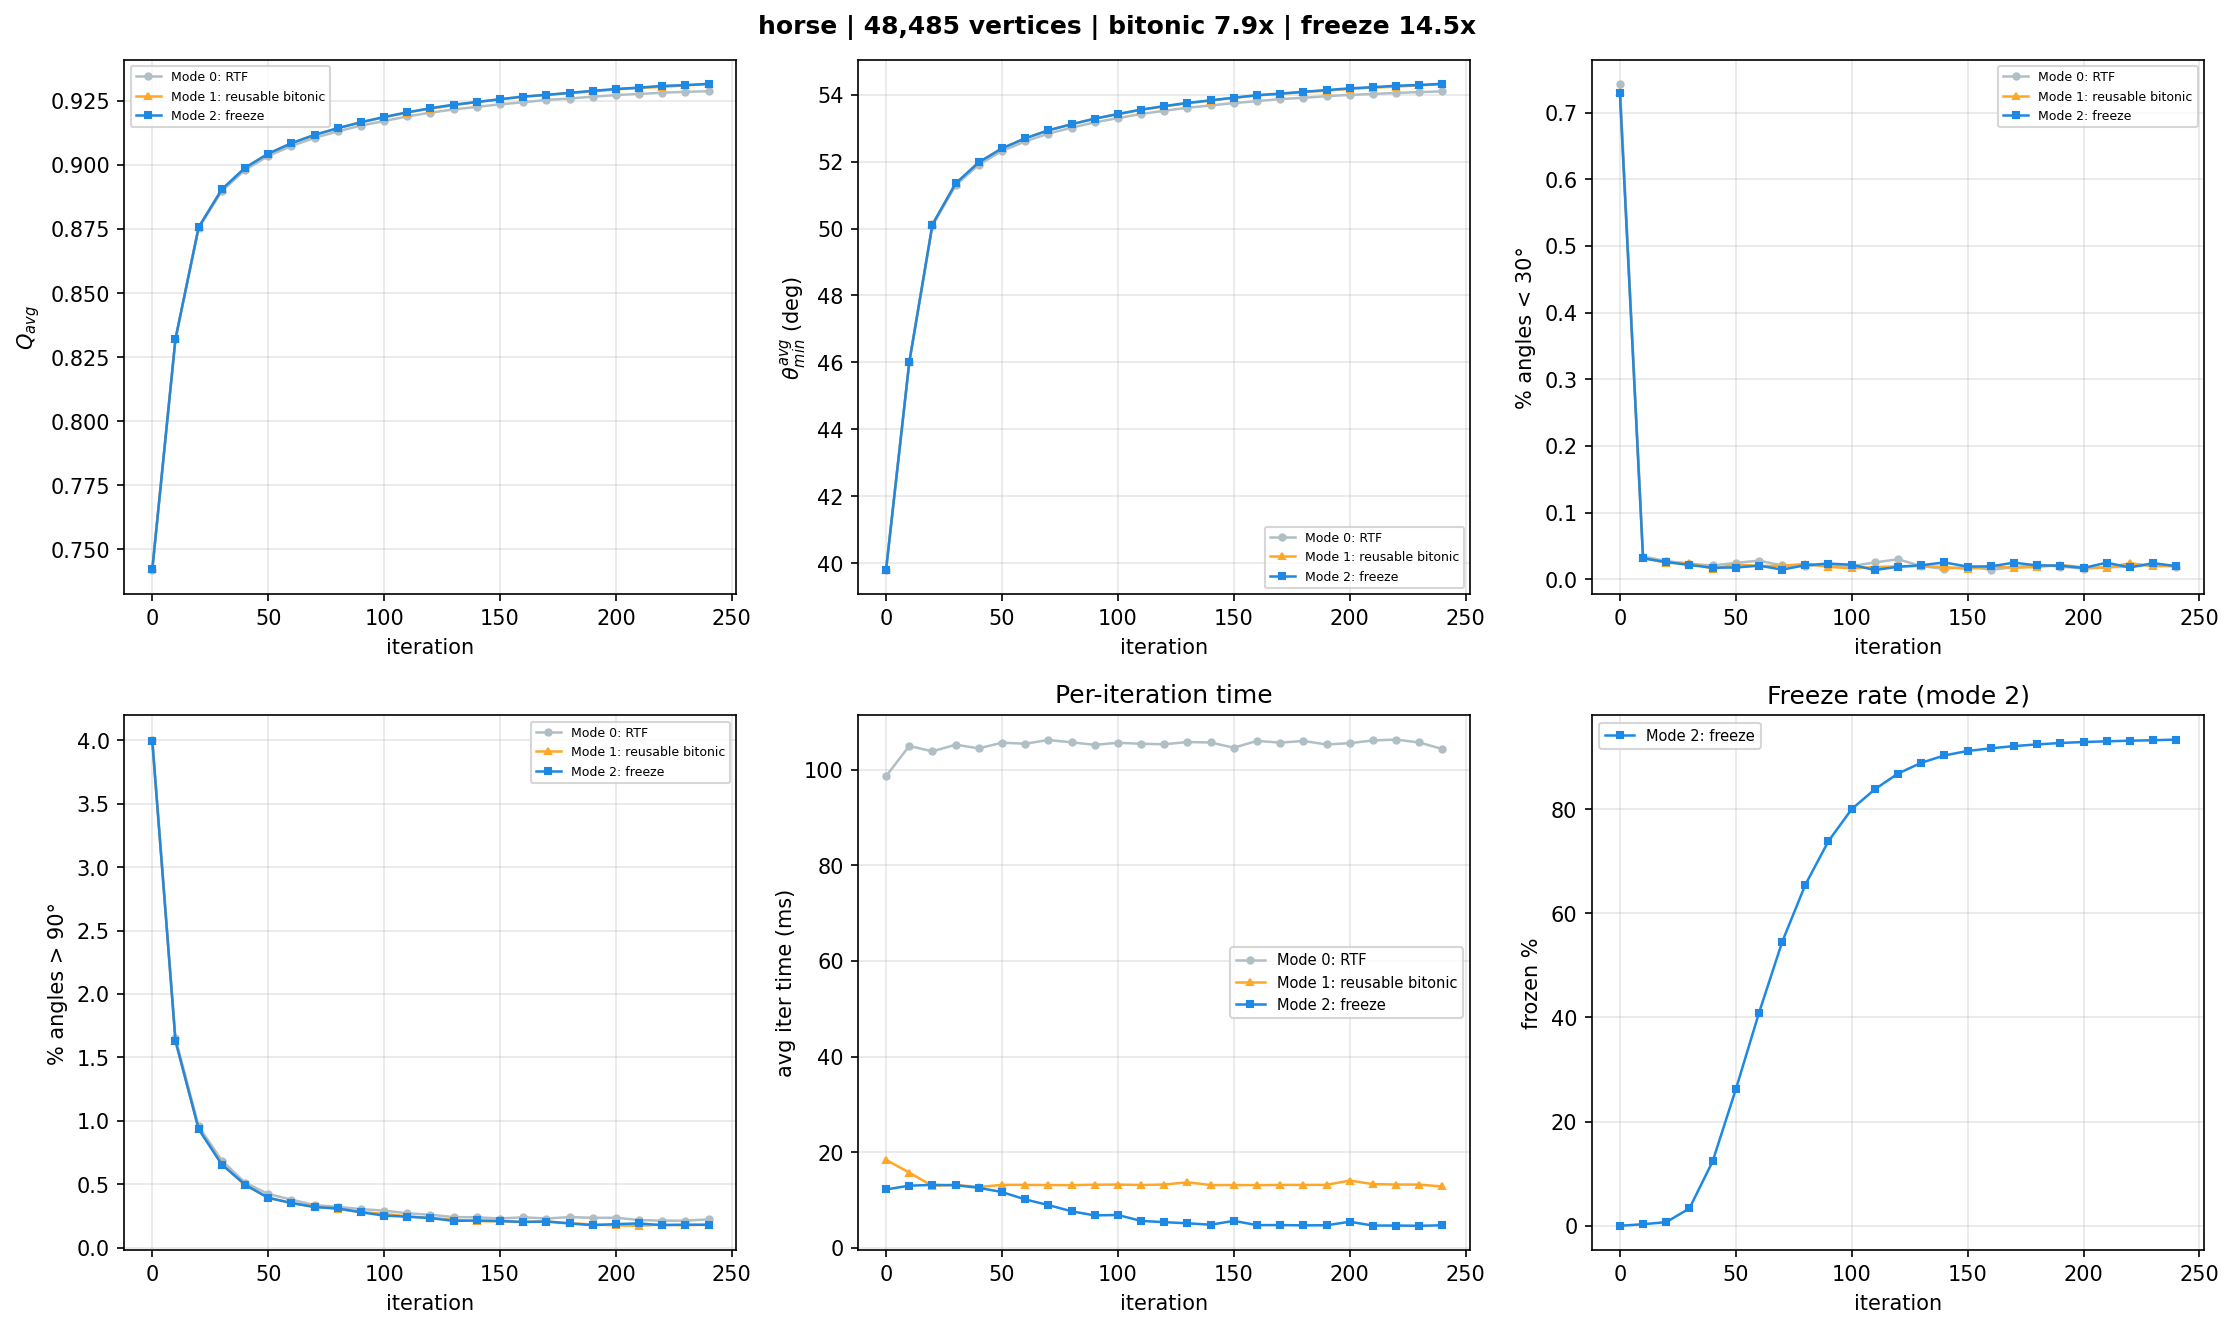
\includegraphics[width=0.32\textwidth]{figs/fig7_three_modes_quality_horse.png}%
\hfill
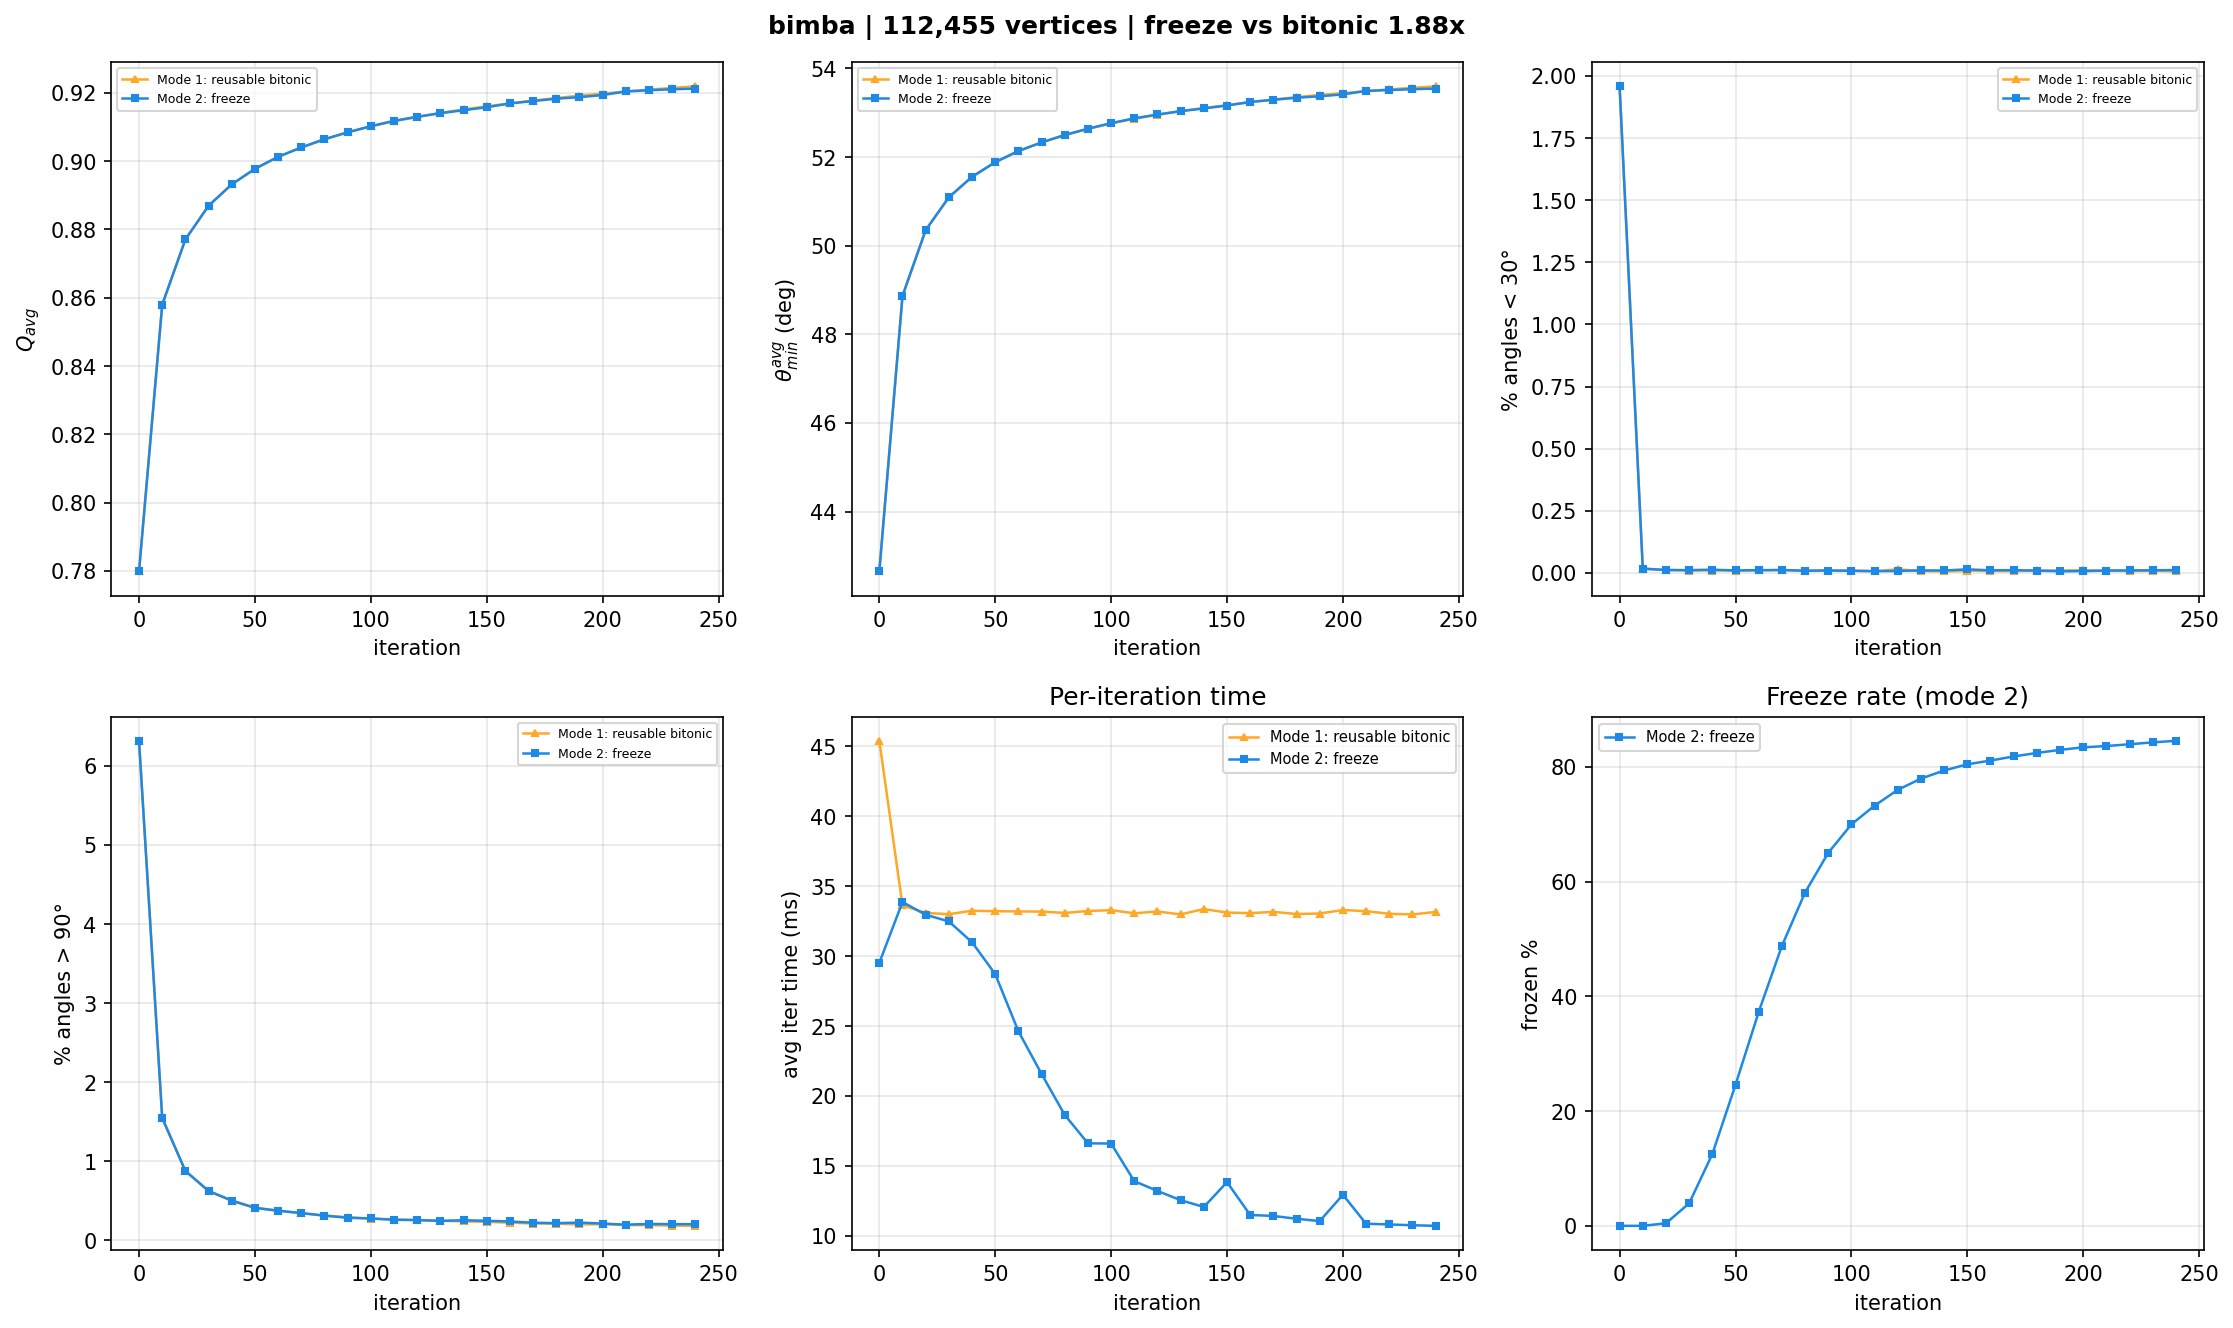
\includegraphics[width=0.32\textwidth]{figs/fig7_three_modes_quality_bimba.png}%
\hfill
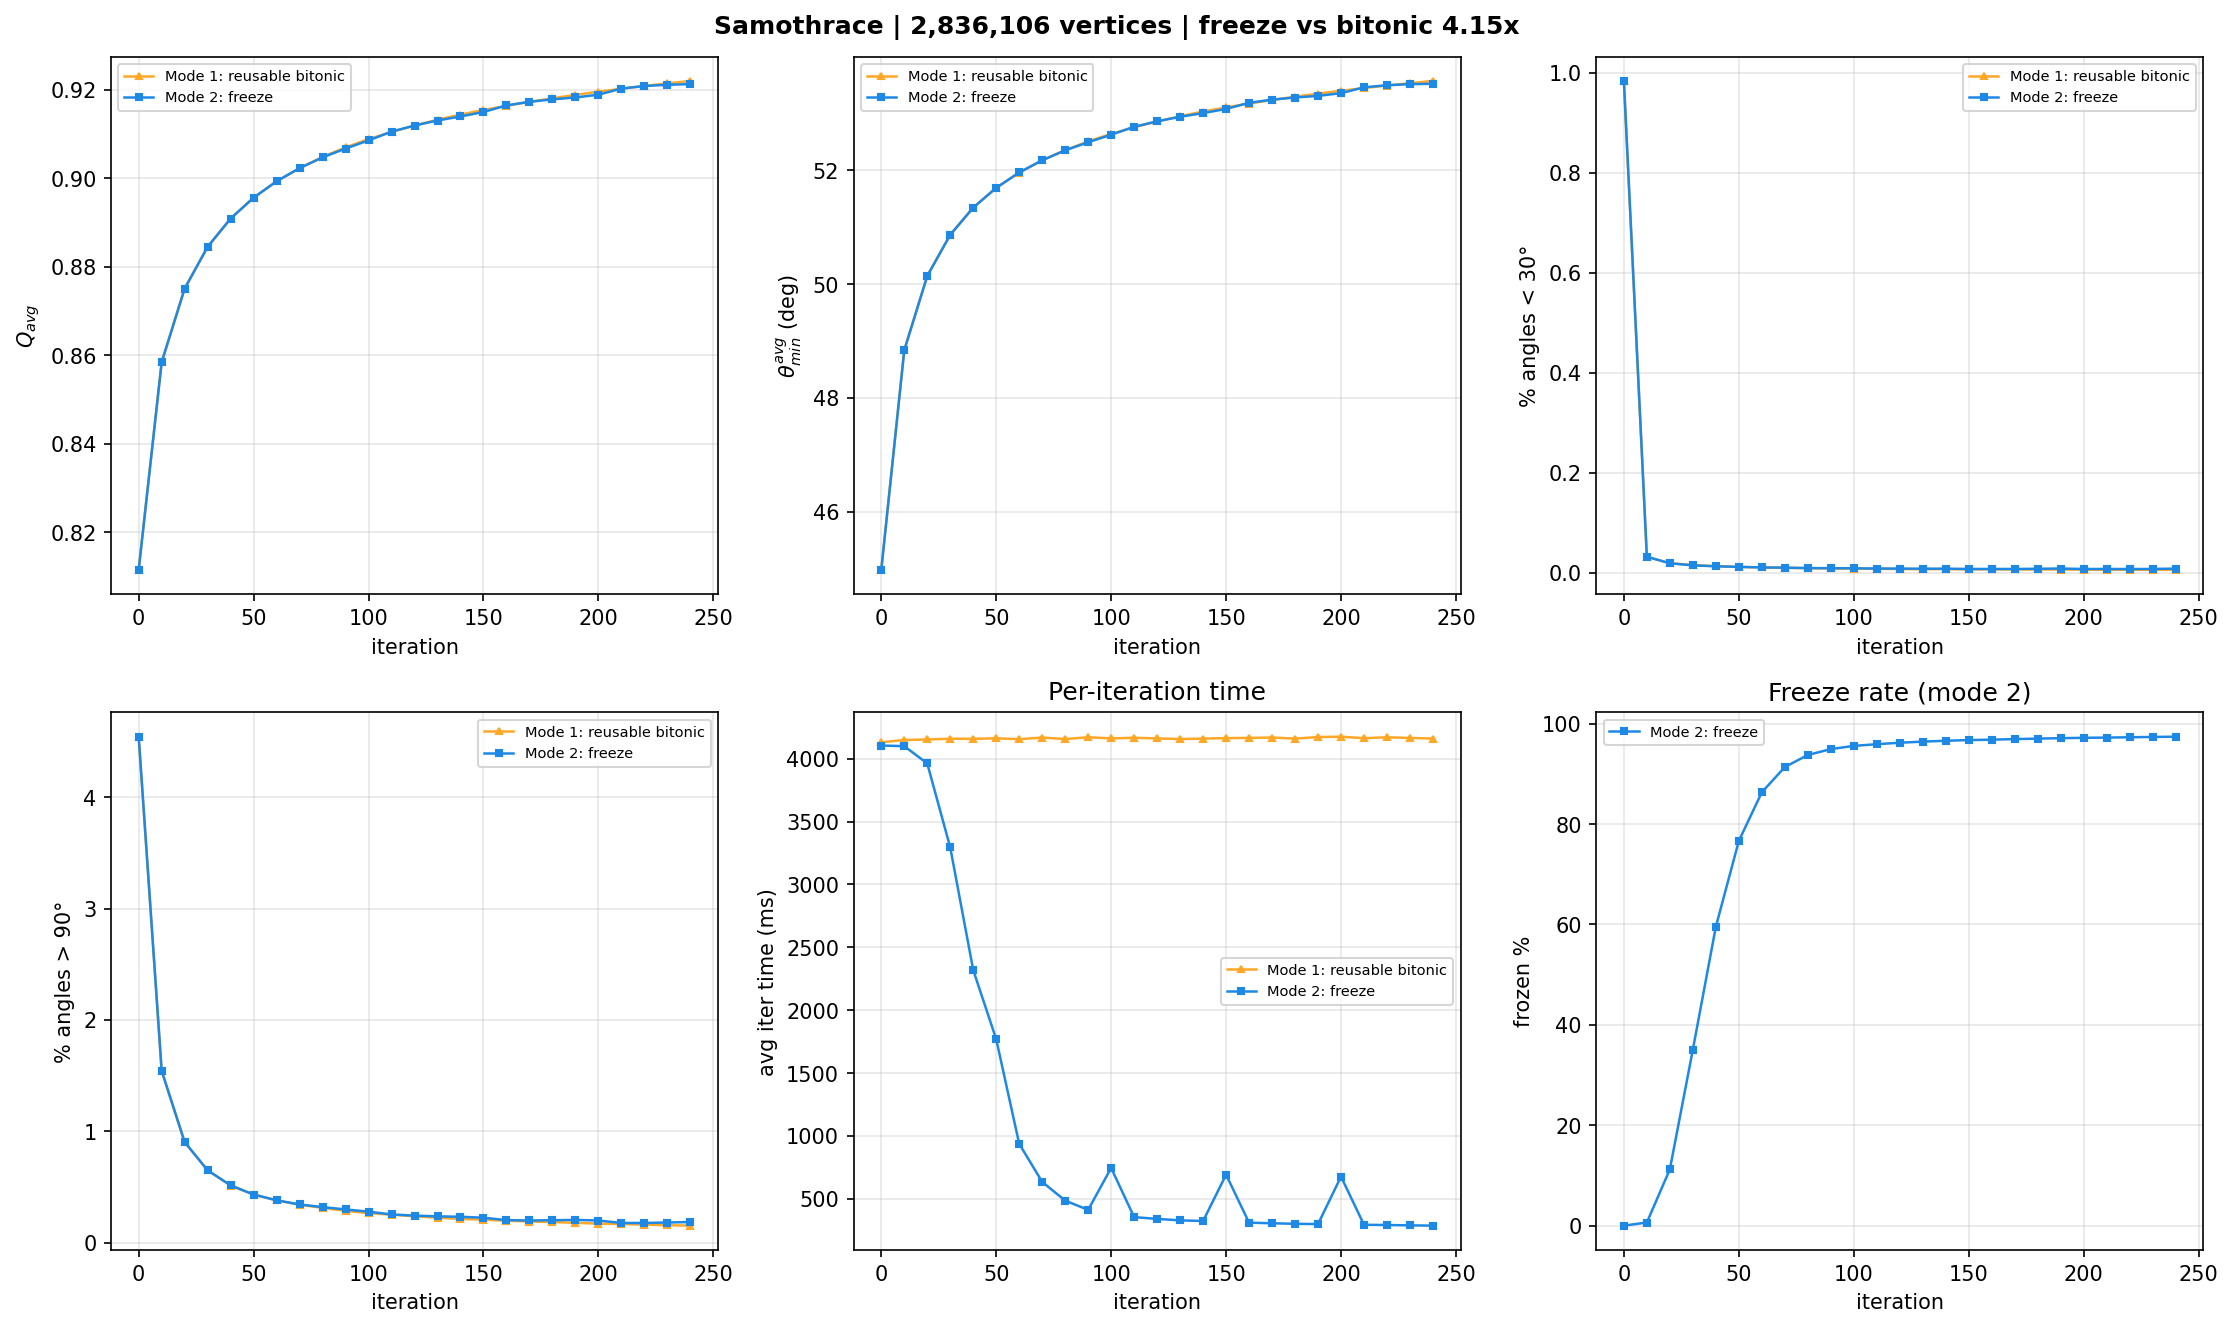
\includegraphics[width=0.32\textwidth]{figs/fig7_three_modes_quality_samothrace.png}
\caption{Quality metrics ($Q_{\mathrm{avg}}$, $\theta_{\min}$, and angle distributions) across RTF~\cite{yao2023rtf}, Mode~1, and Mode~2 over 250 Lloyd iterations on Horse (48K, left), Bimba (112K, center), and Samothrace (2.84M, right). Mode~1 and Mode~2 curves overlap throughout, confirming that the freeze policy does not degrade mesh quality.}
\label{fig:three_modes_quality}
\end{figure*}


\subsection{Ablation: KNN Reuse and Freeze Contributions}
\label{sec:ablation}

To isolate the contribution of each component, we compare RTF~\cite{yao2023rtf}, Mode~1 (reusable KNN only), and Mode~2 (reusable KNN + freeze) across all configurations where each is available.

\textbf{Reusable KNN (RTF $\to$ Mode~1).}
On the three small meshes where RTF is available, replacing RTF's brute-force KNN with our hub-grid bitonic structure yields 5.5--7.9$\times$ speedup. The reusable spatial index avoids RTF's $O(n^2)$ all-pairs scan at every iteration, providing substantial acceleration even without any freezing. The warm-start mechanism further reduces query cost in later iterations when site displacements are small.

\textbf{Freeze policy (Mode~1 $\to$ Mode~2).}
Adding the freeze policy on top of KNN reuse provides an additional speedup that grows consistently with mesh size:
\begin{itemize}
    \item Small meshes (35--50K): 1.6--1.8$\times$, with freeze rates of 80--93\%.
    \item Medium meshes (112--544K): 1.9--2.7$\times$, with freeze rates of 84--98\%.
    \item Large meshes (1.2--2.8M): 3.7--4.2$\times$, with freeze rates of 97--98\%.
\end{itemize}

The two components are synergistic: the freeze policy progressively removes converged sites from the KNN query set, and the reusable KNN structure's frozen-mask compaction ensures that this sparsity translates directly into proportional wall-clock reduction. Without the compaction mechanism, frozen sites would still consume warp occupancy; without the freeze policy, the compaction has nothing to skip.

Quality is preserved across all three modes. \Cref{fig:three_modes_quality} shows $Q_{\mathrm{avg}}$, $\theta_{\min}$, angle distribution metrics, and cumulative timing tracking closely between Mode~1 and Mode~2 throughout iteration on all 11 meshes, confirming that the freeze policy does not degrade mesh quality while the timing curves diverge progressively as the freeze rate grows.

\subsection{Freeze Behavior and Quality Preservation}
\label{sec:freeze_behavior}

We examine the freeze policy's behavior in detail to verify that the curvature-adaptive design achieves high freeze rates without compromising output quality.

\textbf{Progressive freezing.}
The freeze rate rises monotonically over the course of iteration. On medium meshes, sites in flat regions (Tier~0--1) begin freezing around iteration 30--50, once the streak requirement of 10--15 consecutive passes is met. Sites in moderate-curvature regions (Tier~2--3) follow at iteration 60--100. Sites near sharp features (Tier~4) freeze late or remain active throughout, as their longer streak requirements (25--30 iterations) and stricter KNN stability checks reflect the genuine difficulty of convergence in these regions. The final freeze rate on medium meshes ranges from 84\% (Bimba) to 98\% (Igea, which is predominantly smooth).

On large meshes, the freeze rate exceeds 97\% on all three test cases. At high sampling density, the surface is dominated by flat regions that gain proportionally more sites, all of which converge early and pass the freeze test quickly. The small fraction of sites near sharp features---typically under 3\% of the total at million-vertex scale---remains active, preserving detail fidelity.

\textbf{Quality preservation.}
Across all 11 meshes, the quality metrics of Mode~2 (freeze) track those of Mode~1 (no freeze) within negligible margin throughout iteration. The $Q_{\mathrm{avg}}$ curves overlap to within 0.1\%, and the angle distribution metrics (\%$< 30°$, \%$> 90°$) show no systematic divergence. This confirms that the dual-gate test with curvature-scaled streaks successfully avoids false freezing: only sites whose position and neighborhood have genuinely stabilized are removed from KNN queries.

\textbf{Per-iteration time reduction.}
\Cref{fig:time_breakdown} shows the per-iteration time breakdown by pipeline stage at iterations 0, 50, 100, and 200. As freezing progresses, total per-iteration time drops by $3$--$4\times$: Horse falls from 18.6ms to 5.7ms, Armadillo from 51.4ms to 16.8ms, and Happy Buddha from 284ms to 71ms. The KNN query (red) and KNN-to-mesh stages (orange) shrink in absolute terms as frozen sites are compacted out of the query set, while clipping, centroid, and reprojection (which run for all sites) remain roughly constant. KNN's share of per-iteration cost ranges from 24--32\% at iteration~0 to 42--58\% at iteration~200 --- it remains the largest single stage even after freezing, confirming that further KNN optimization would compound with the freeze policy.

\begin{figure*}[t]
\centering
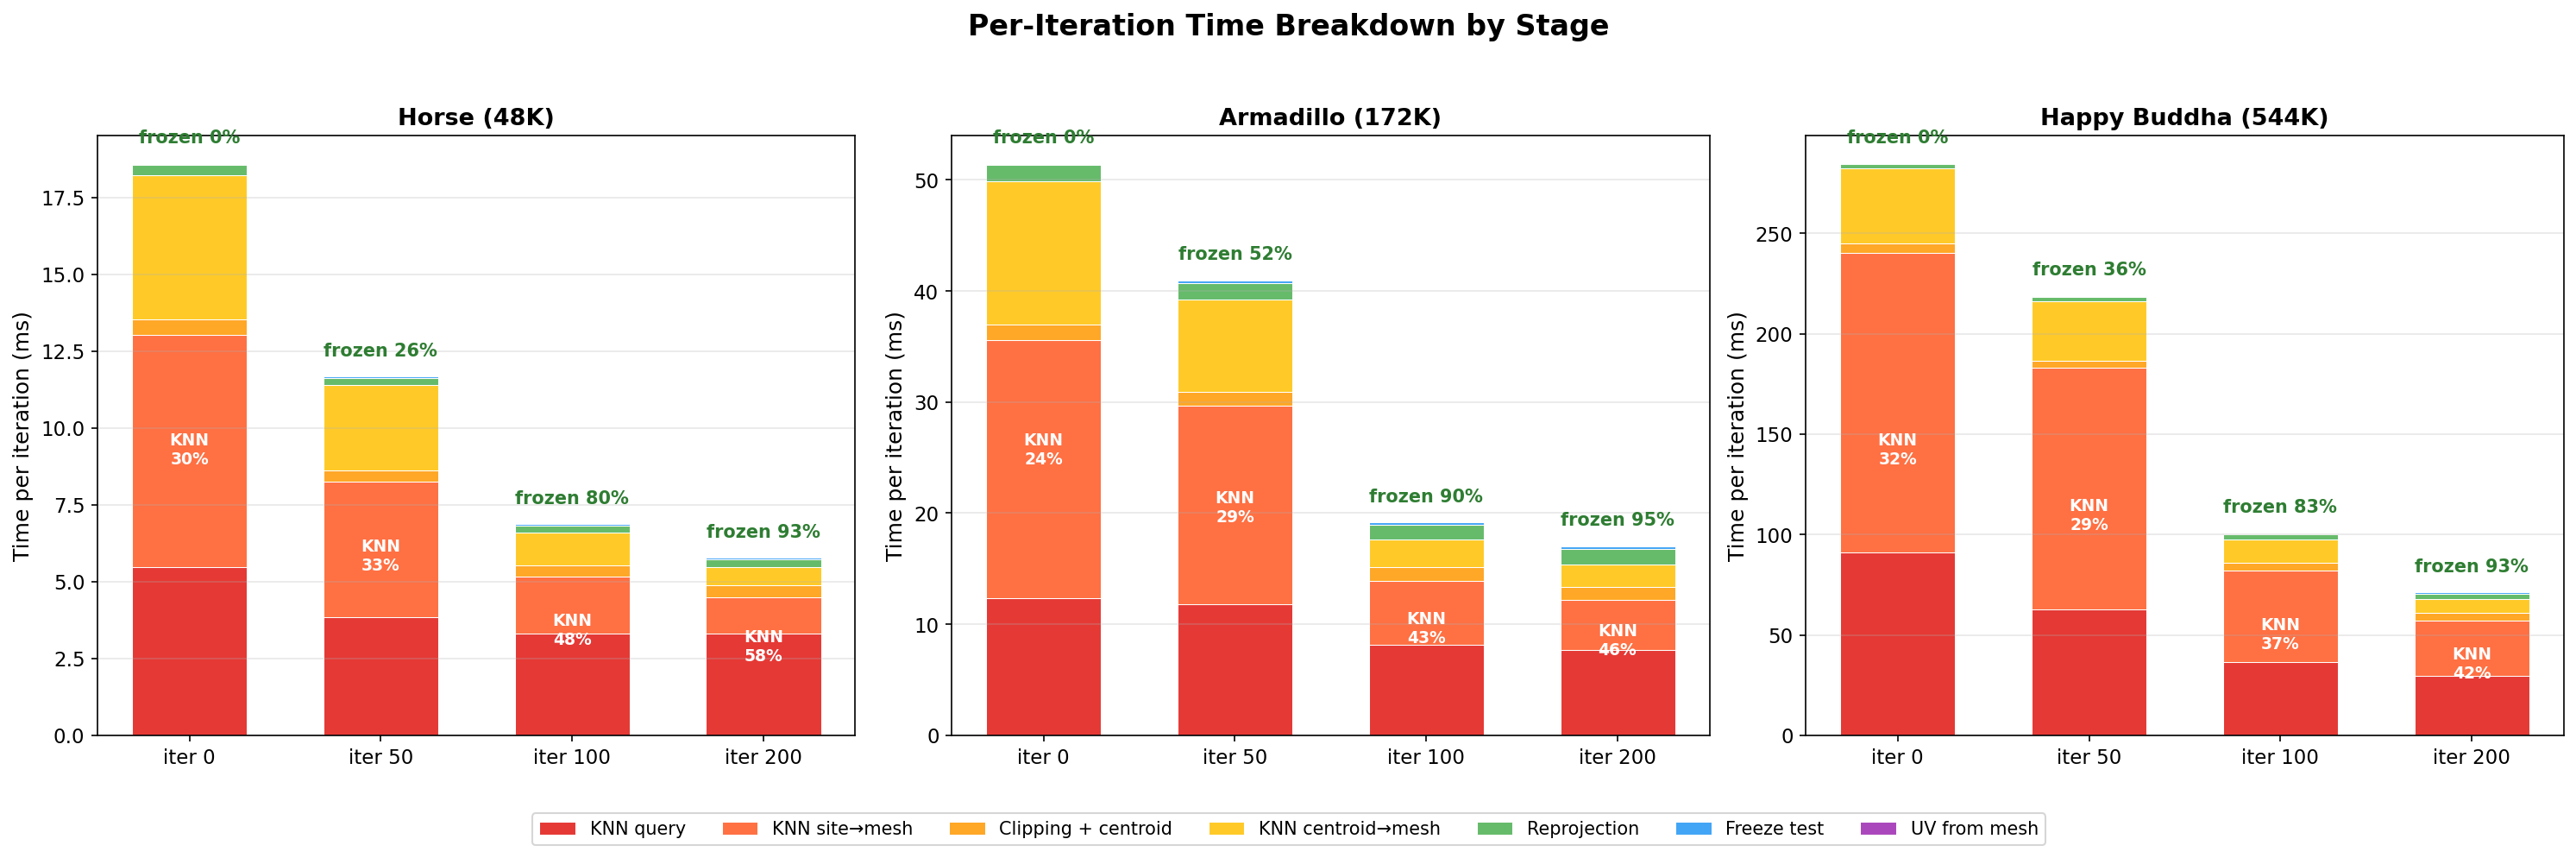
\includegraphics[width=\textwidth]{figs/fig13_time_breakdown.png}
\caption{Per-iteration time breakdown by pipeline stage at iterations 0, 50, 100, and 200 for Horse (48K), Armadillo (172K), and Happy Buddha (544K). As the freeze rate grows (green labels), total iteration time shrinks by $3$--$4\times$. KNN query time (red) decreases in absolute terms as frozen sites are compacted out, while non-KNN stages remain roughly constant.}
\label{fig:time_breakdown}
\end{figure*}

\subsection{Comparison with CPU Baselines}
\label{sec:cpu_comparison}

\Cref{fig:all_methods} compares all six methods on the Horse mesh (48K vertices), the smallest scale at which all baselines are available. CGAL isotropic remeshing~\cite{botsch2004remeshing} and ACVD~\cite{valette2008acvd} are strictly dominated by Geogram in both quality and speed: CGAL produces $Q_{\mathrm{avg}} \approx 0.860$ at $7.0$s (vs.\ Geogram's $0.929$ at $18.2$s), while ACVD achieves $Q_{\mathrm{avg}} \approx 0.880$ at $13.3$s. Neither method is competitive with any GPU mode. We therefore use Geogram RVD-CVT~\cite{levy2010lp}---the state-of-the-art CPU implementation based on exact restricted Voronoi diagrams with Delaunay triangulation---as our primary baseline for the remainder of this section.

\begin{figure*}[t]
\centering
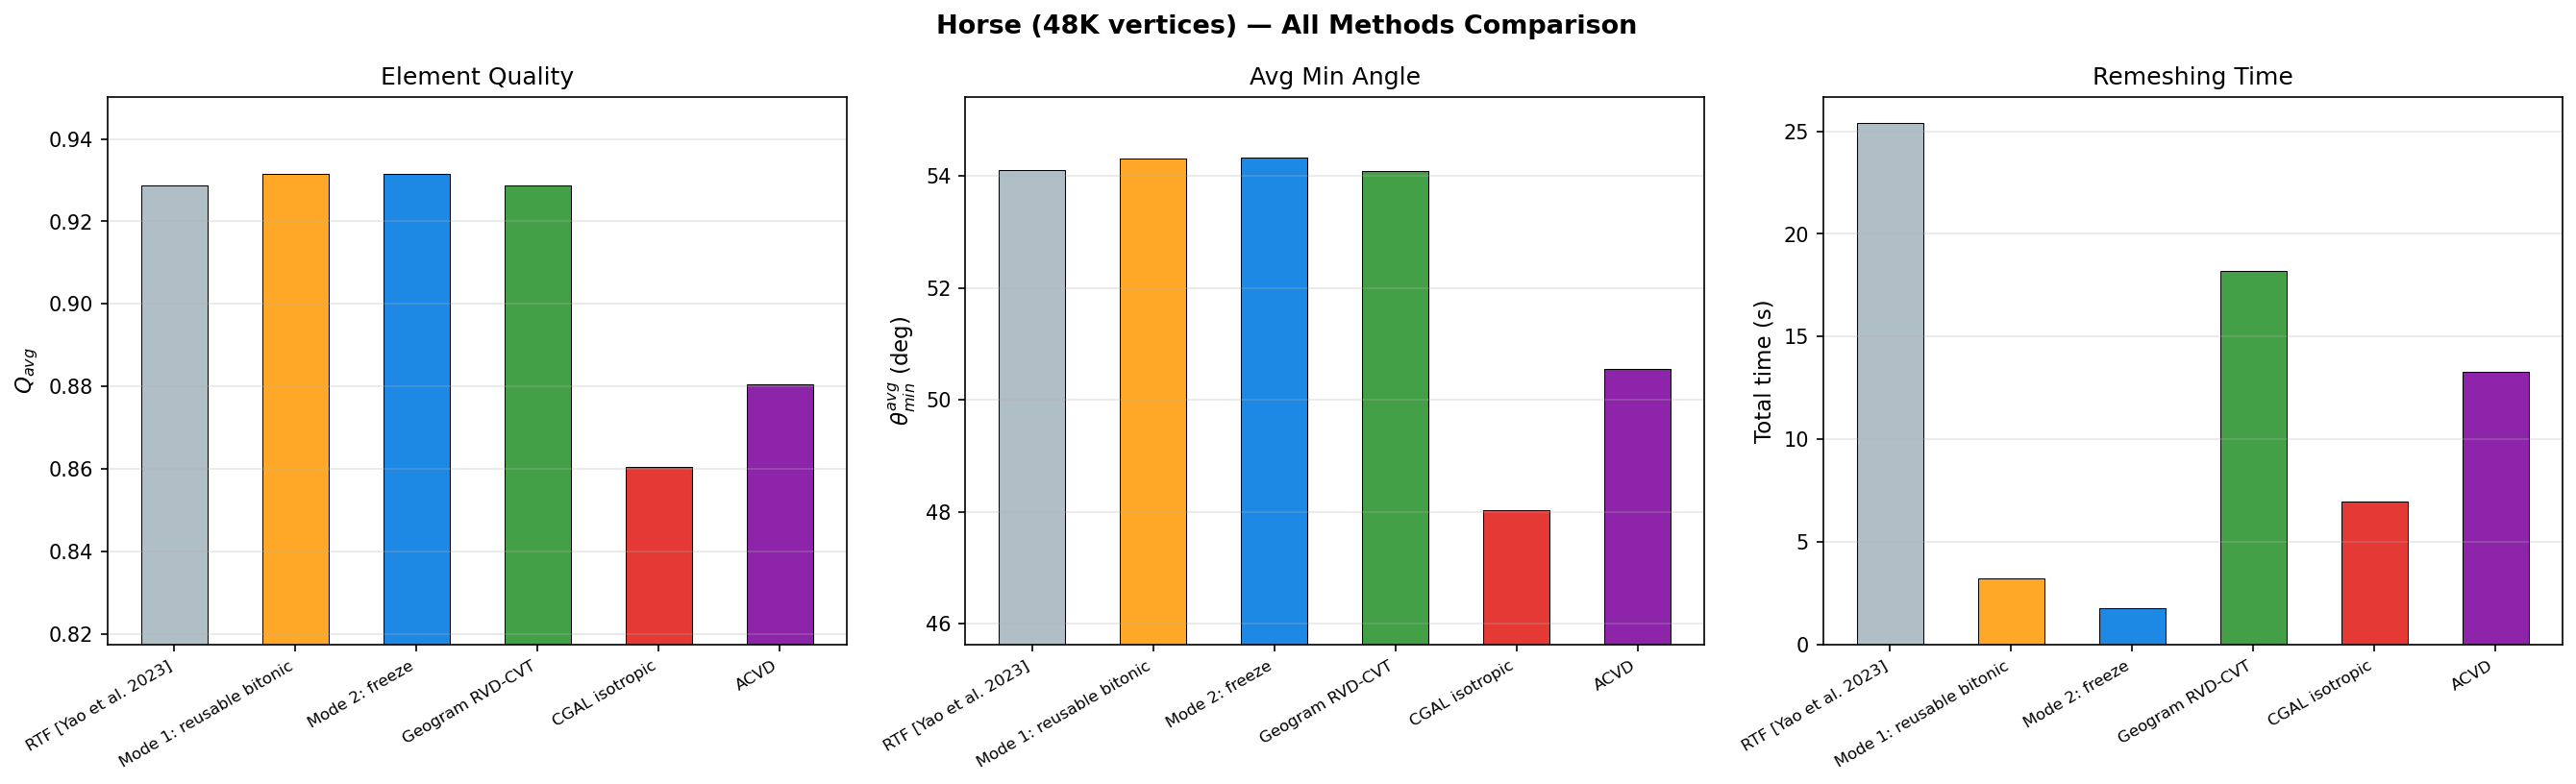
\includegraphics[width=\textwidth]{figs/fig10_all_methods_horse.png}
\caption{All-methods comparison on Horse (48K vertices). CGAL isotropic and ACVD produce substantially lower element quality ($Q_{\mathrm{avg}} \approx 0.86$--$0.88$) at 4--8$\times$ higher runtime than Geogram RVD-CVT, and are not competitive with any GPU mode. Geogram achieves the highest quality ($Q_{\mathrm{avg}} = 0.929$) but at $10.4\times$ the runtime of Mode~2.}
\label{fig:all_methods}
\end{figure*}

For a fair comparison, Geogram is configured with 250 Lloyd iterations (matching our iteration count) and $n_{\mathrm{samples}} = n_{\mathrm{vertices}}$ (matching our site count). \Cref{fig:baseline_comparison} summarizes element quality, average minimum angle, and total remeshing time side by side for representative meshes at three scales.

On small meshes (35--50K vertices), Mode~2 is 8.0--10.4$\times$ faster than Geogram while achieving comparable quality ($Q_{\mathrm{avg}} \approx 0.926$ vs.\ Geogram's 0.929). As shown in the Horse panel of \Cref{fig:baseline_comparison}, all four methods produce nearly identical $Q_{\mathrm{avg}}$ and $\theta_{\min}^{\mathrm{avg}}$, while Mode~2's runtime is an order of magnitude smaller than both RTF and Geogram. The quality gap of approximately 0.3\% is inherent to the tangent-plane approximation used by all KNN-based CVT methods versus Geogram's exact RVD computation; it is not caused by freezing, as Mode~1 (without freeze) produces the same quality.

On medium meshes (112--544K), Mode~2 maintains a 3.1--8.5$\times$ speedup over Geogram. The Bimba panel of \Cref{fig:baseline_comparison} illustrates that Mode~2 achieves quality within 1\% of Geogram at $8.5\times$ lower runtime. At the largest medium mesh (happy\_vrip, 544K), Geogram takes 117 seconds while Mode~2 completes in 27 seconds, a 4.3$\times$ advantage (\Cref{fig:baseline_comparison}, right). The freeze policy is essential at this scale: Mode~1 alone achieves only 1.8$\times$ over Geogram, while Mode~2's freeze-driven compaction provides the additional factor needed to maintain a clear advantage.

On large meshes (1.2--2.8M vertices), Geogram is not run. Extrapolating from its observed $O(n \log n)$ per-iteration scaling---117 seconds at 544K vertices---we estimate a runtime on the order of 700--800 seconds for 2.8M vertices (Samothrace). Mode~2 completes the same mesh in 241 seconds, approximately 3$\times$ faster than the extrapolated baseline. RTF is also not run at this scale; its $O(n^2)$ KNN cost would require hours. At million-vertex scale, only Mode~2 with freeze-aware KNN reuse produces results within a practical time budget.

\begin{figure*}[t]
\centering
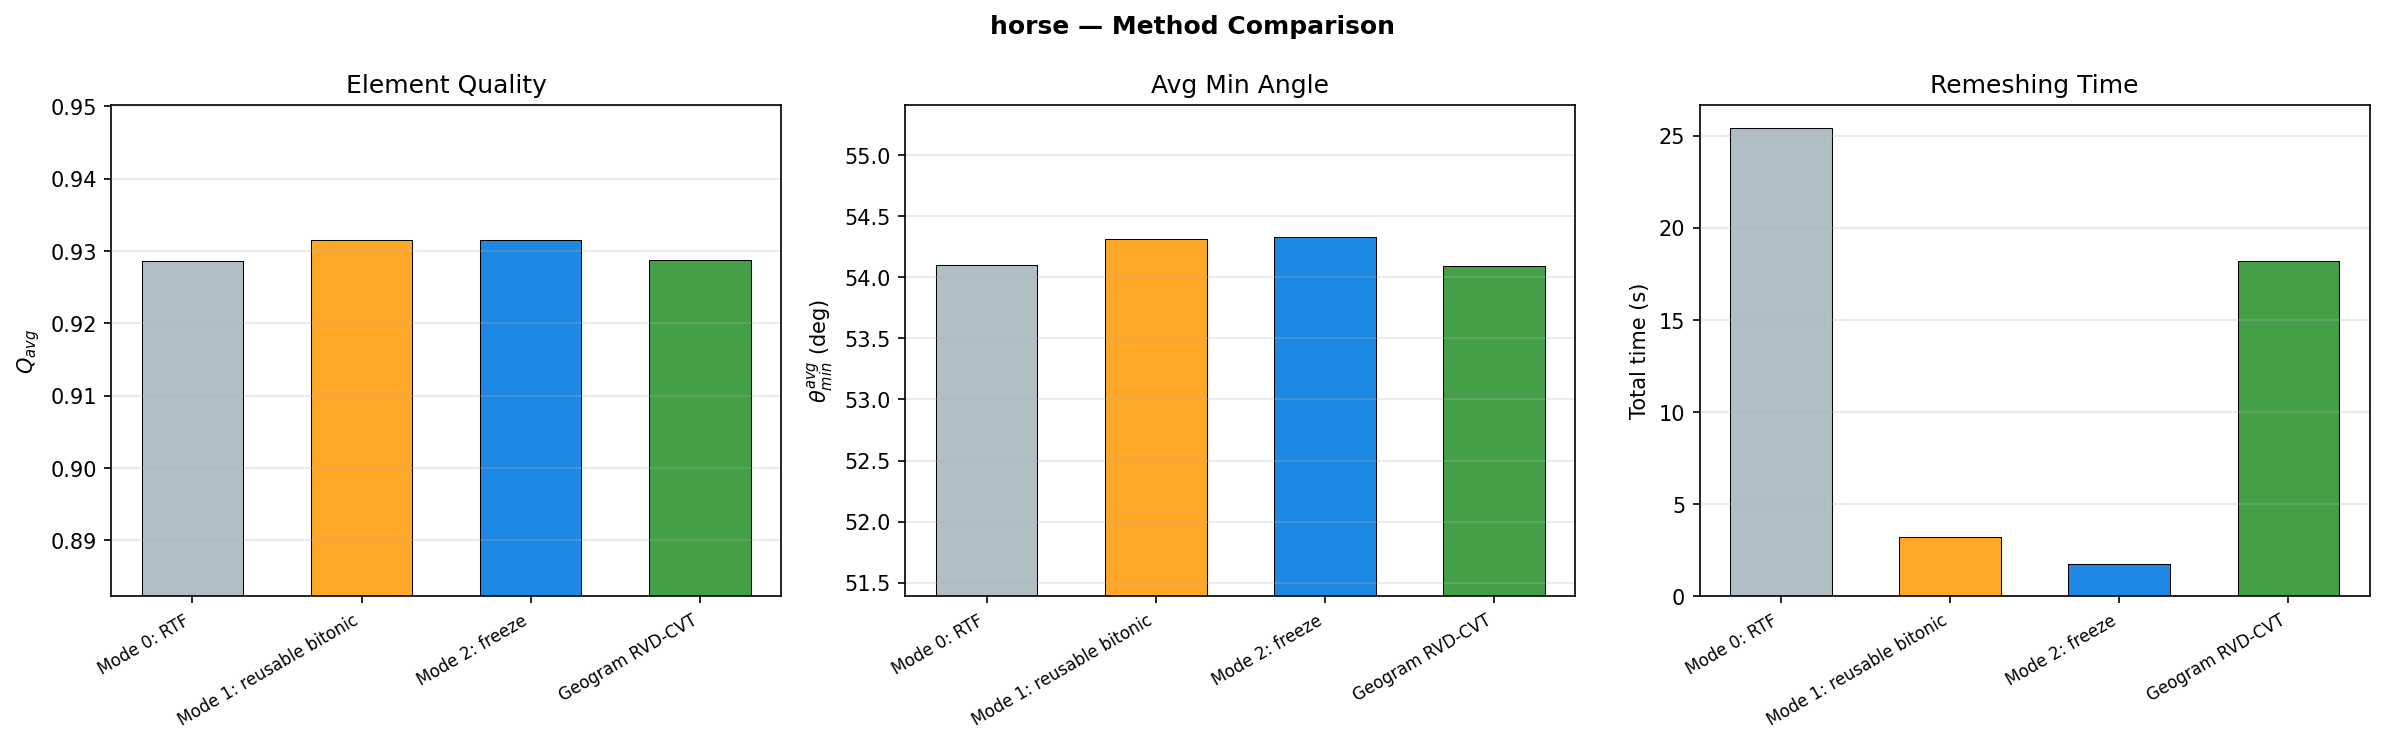
\includegraphics[width=0.32\textwidth]{figs/fig9_baseline_comparison_horse.png}%
\hfill
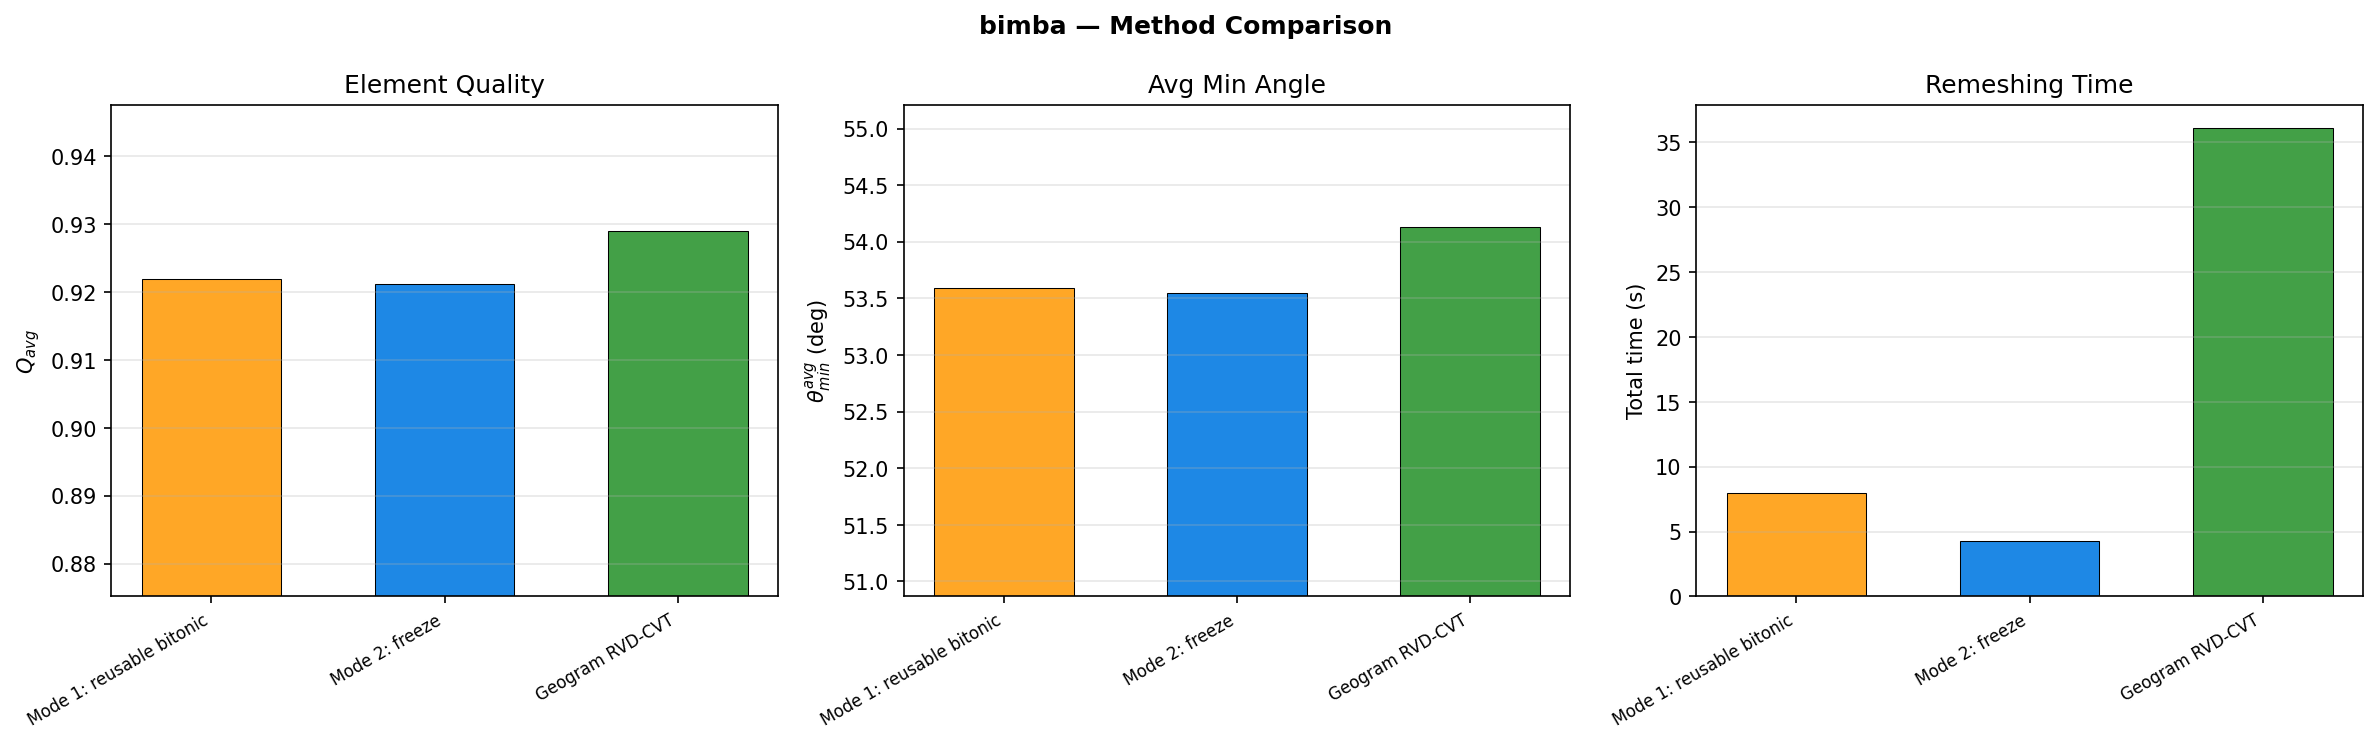
\includegraphics[width=0.32\textwidth]{figs/fig9_baseline_comparison_bimba.png}%
\hfill
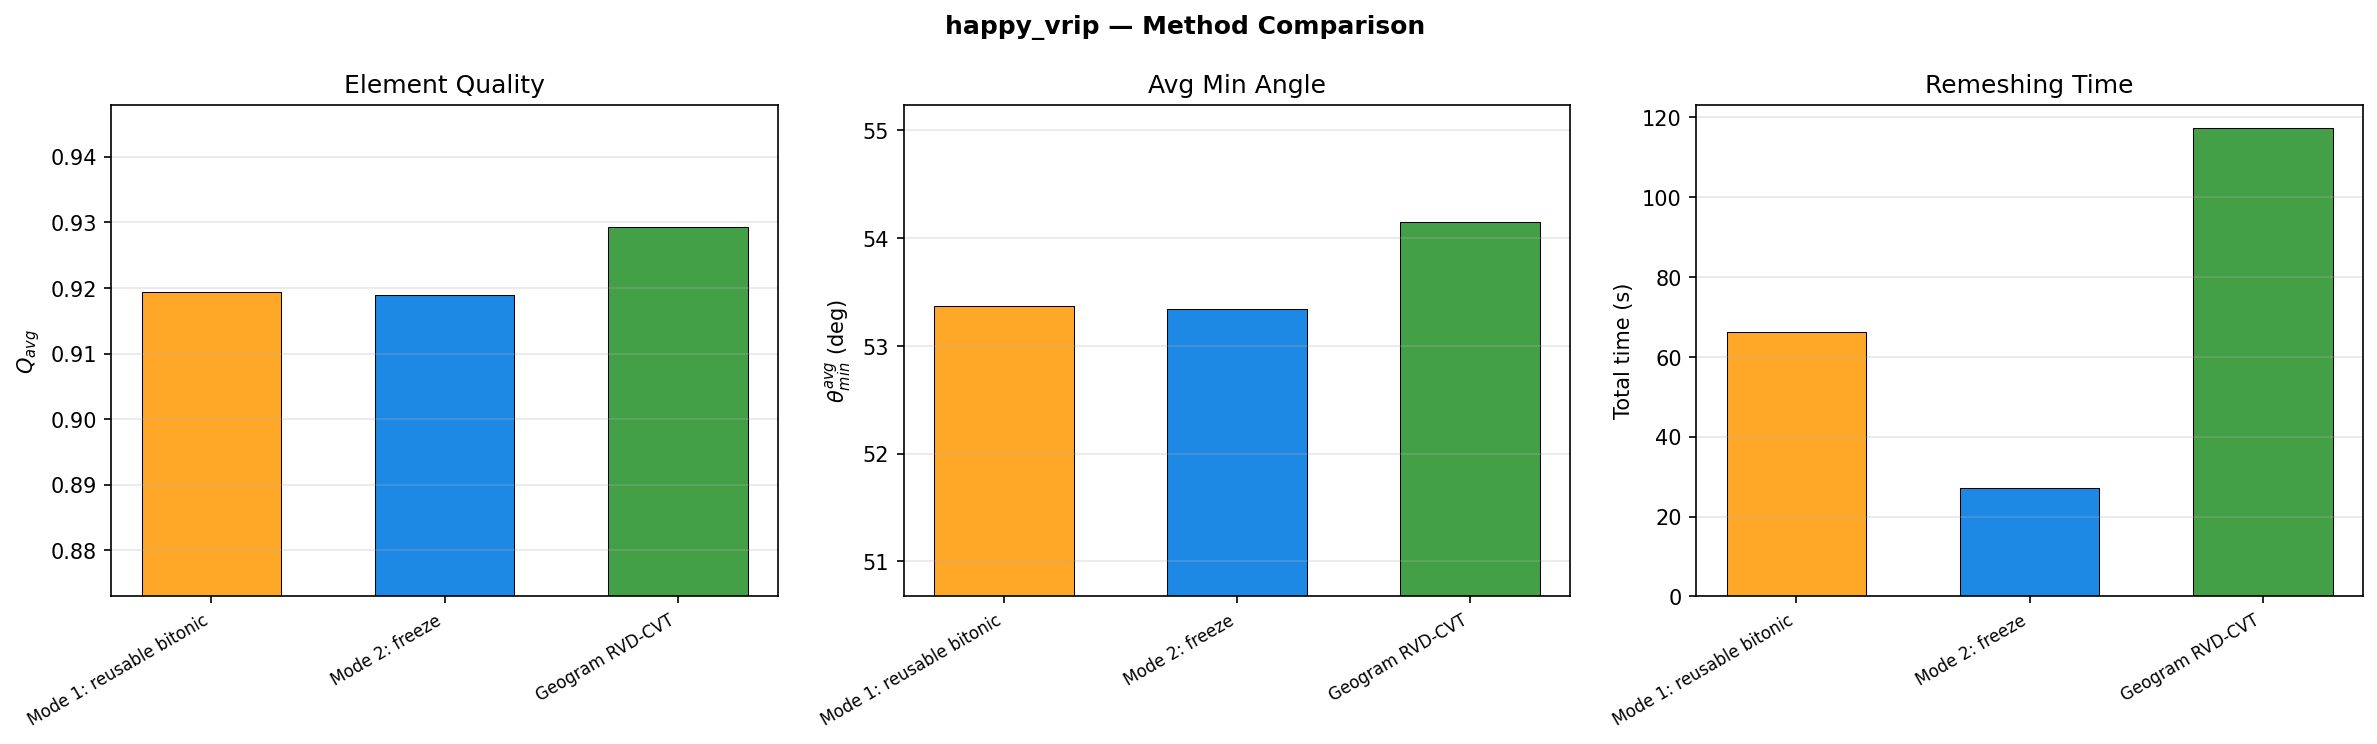
\includegraphics[width=0.32\textwidth]{figs/fig9_baseline_comparison_happy_vrip.png}
\caption{Baseline comparison of element quality ($Q_{\mathrm{avg}}$), average minimum angle ($\theta_{\min}^{\mathrm{avg}}$), and total remeshing time across methods on Horse (48K, left), Bimba (112K, center), and Happy Buddha (544K, right). All methods produce comparable quality, while Mode~2 achieves 8--10$\times$ lower runtime than Geogram RVD-CVT across all scales.}
\label{fig:baseline_comparison}
\end{figure*}

\subsection{Memory Footprint}
\label{sec:memory}

\Cref{tab:memory} reports peak GPU memory measured via \texttt{nvidia-smi} during Mode~2 execution. Memory scales sublinearly with vertex count: Horse (48K) uses 566\,MiB while Samothrace (2.84M) uses 5,494\,MiB---a $58\times$ increase in vertices for only $9.7\times$ more memory. This is because the dominant allocations (Voronoi polygon buffers at $N \times 256$ slots) use CUDA virtual memory with lazy physical backing; only touched pages consume physical VRAM. On our 8\,GB GPU, the practical limit is approximately 3.5--4M vertices, beyond which the working set exceeds available VRAM.

\begin{table}[t]
\centering
\caption{Peak GPU memory (measured) during Mode~2 execution on an RTX 4070 Laptop (8\,GB VRAM).}
\label{tab:memory}
\small
\begin{tabular}{lrr}
\hline
Mesh & Vertices & Peak GPU (MiB) \\
\hline
stanford-bunny & 34{,}834 & 566 \\
horse & 48{,}485 & 566 \\
Armadillo & 172{,}974 & 1{,}524 \\
dragon\_vrip & 437{,}645 & 3{,}638 \\
happy\_vrip & 543{,}652 & 4{,}502 \\
Samothrace & 2{,}836{,}106 & 5{,}494 \\
\hline
\end{tabular}
\end{table}

\subsection{Parameter Sensitivity}
\label{sec:sensitivity}

We vary five freeze-policy parameters one at a time on Horse (48K) and Armadillo (172K) to assess robustness. The results reveal a clean separation: \emph{periodic KNN refresh} controls correctness, while all other parameters control only efficiency.

\textbf{Refresh interval $R$} (\Cref{fig:sensitivity_refresh}) is the only parameter whose extreme setting degrades quality: disabling refresh entirely ($R = \infty$) reduces Armadillo $Q_{\mathrm{avg}}$ from 0.933 to 0.925, as stale KNN accumulates without correction. For any finite $R \leq 200$, quality is preserved within 0.001. Runtime is unaffected by $R$---refresh overhead is ${\sim}2\%$ of iteration cost. This confirms that refresh acts as a low-cost correctness safety net.

\textbf{Streak lengths} (\Cref{fig:sensitivity_streak}) control how aggressively sites freeze. Short streaks $\{5, \ldots, 15\}$ achieve 97\% freeze rate and $1.4\times$ faster runtime than long streaks $\{20, \ldots, 40\}$ (86\% freeze). Quality varies by less than 0.001 across all settings because refresh bounds accumulated error from any premature freezing.

\textbf{NV tier boundaries, Kc/K ratio, and warmup $T_0$} have minimal effect. NV boundaries and warmup produce $<$0.1\% variation in all metrics. Stricter Kc/K (uniform 100\%) slows runtime by $1.5\times$ without improving quality---the per-tier default balances gate strictness with freeze efficiency.

The practical consequence is that the method requires no per-mesh tuning. Refresh provides the correctness guarantee; the remaining parameters have a wide safe operating range where quality is invariant and only runtime varies modestly.

\begin{figure*}[t]
\centering
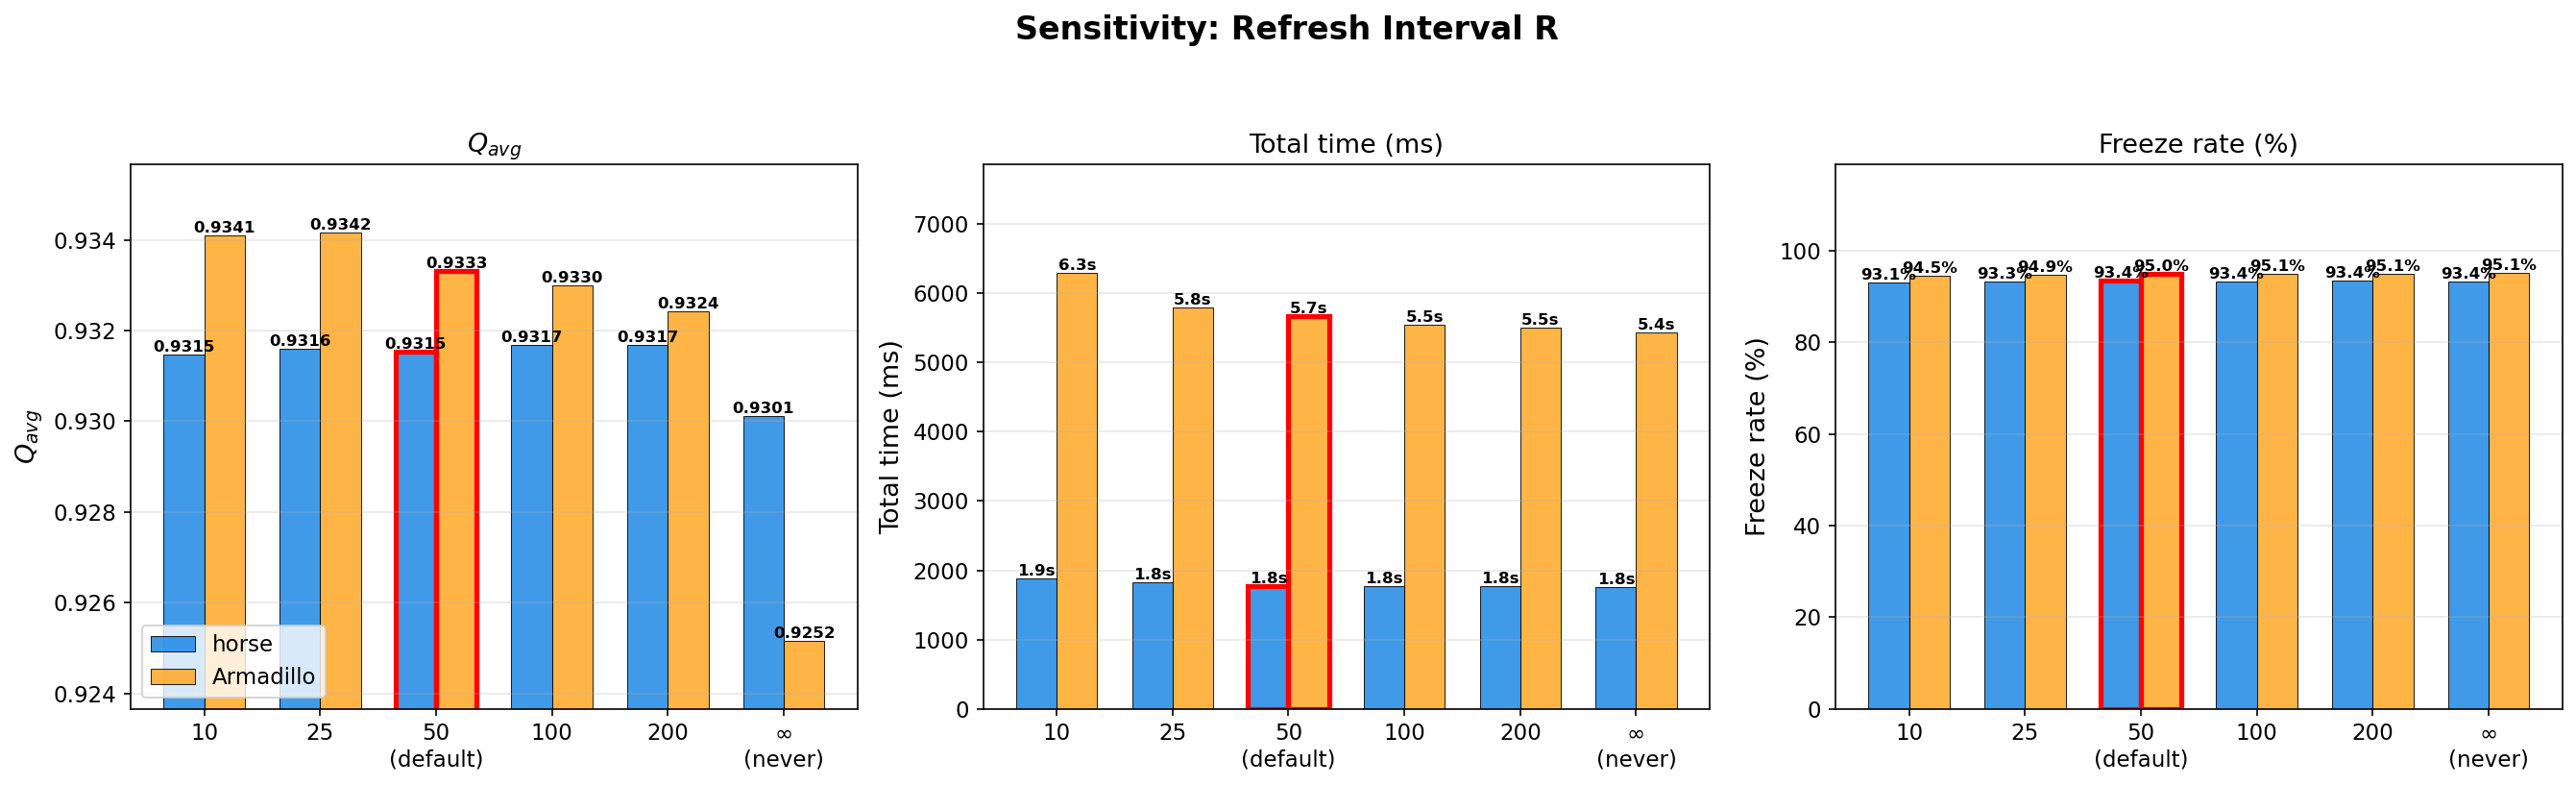
\includegraphics[width=\textwidth]{figs/fig11_sensitivity_refresh.png}
\caption{Sensitivity to refresh interval $R$. Quality ($Q_{\mathrm{avg}}$) is stable for $R \leq 200$ but degrades at $R = \infty$ (no refresh), confirming that periodic refresh is essential for correctness. Runtime and freeze rate are unaffected by $R$. Red border marks the default ($R = 50$).}
\label{fig:sensitivity_refresh}
\end{figure*}

\begin{figure*}[t]
\centering
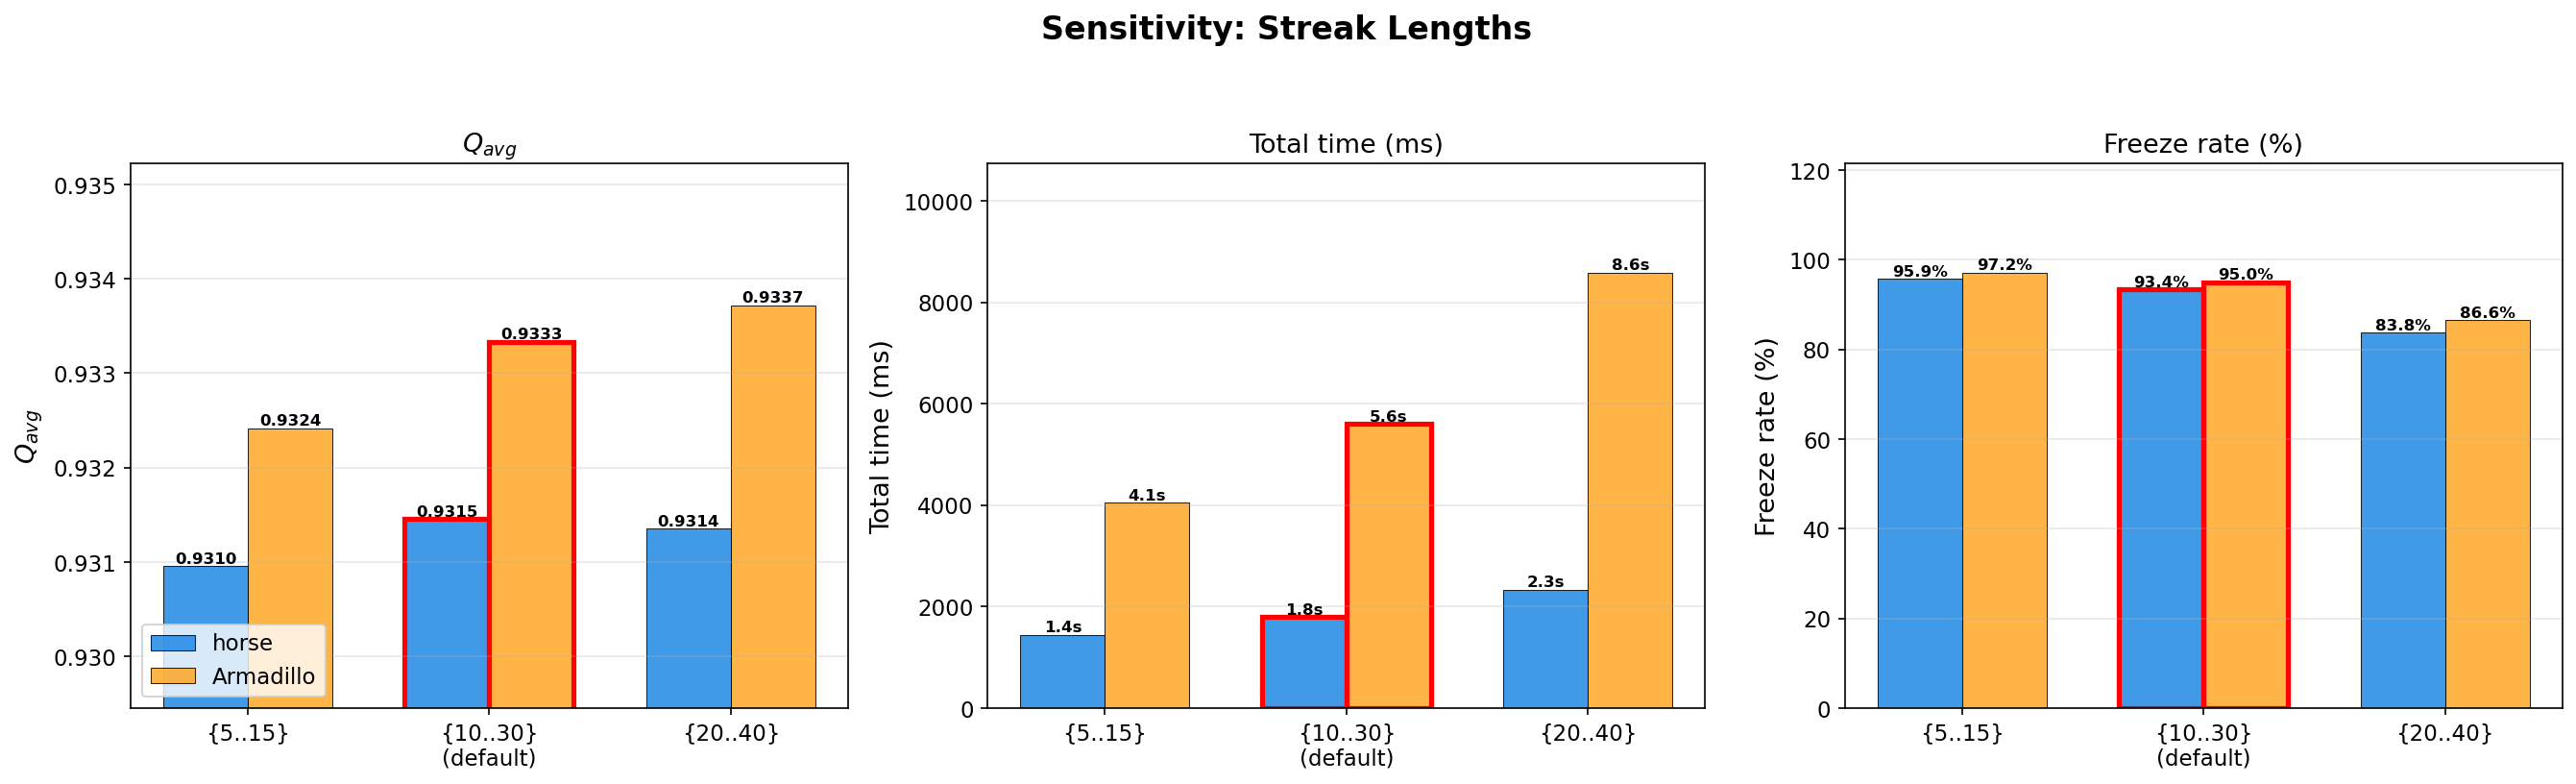
\includegraphics[width=\textwidth]{figs/fig12_sensitivity_streak.png}
\caption{Sensitivity to streak lengths. Shorter streaks freeze more sites earlier (97\% vs 87\%), reducing runtime, with negligible quality difference ($<$0.001). Periodic refresh bounds error from aggressive freezing.}
\label{fig:sensitivity_streak}
\end{figure*}

\begin{figure*}[t]
\centering
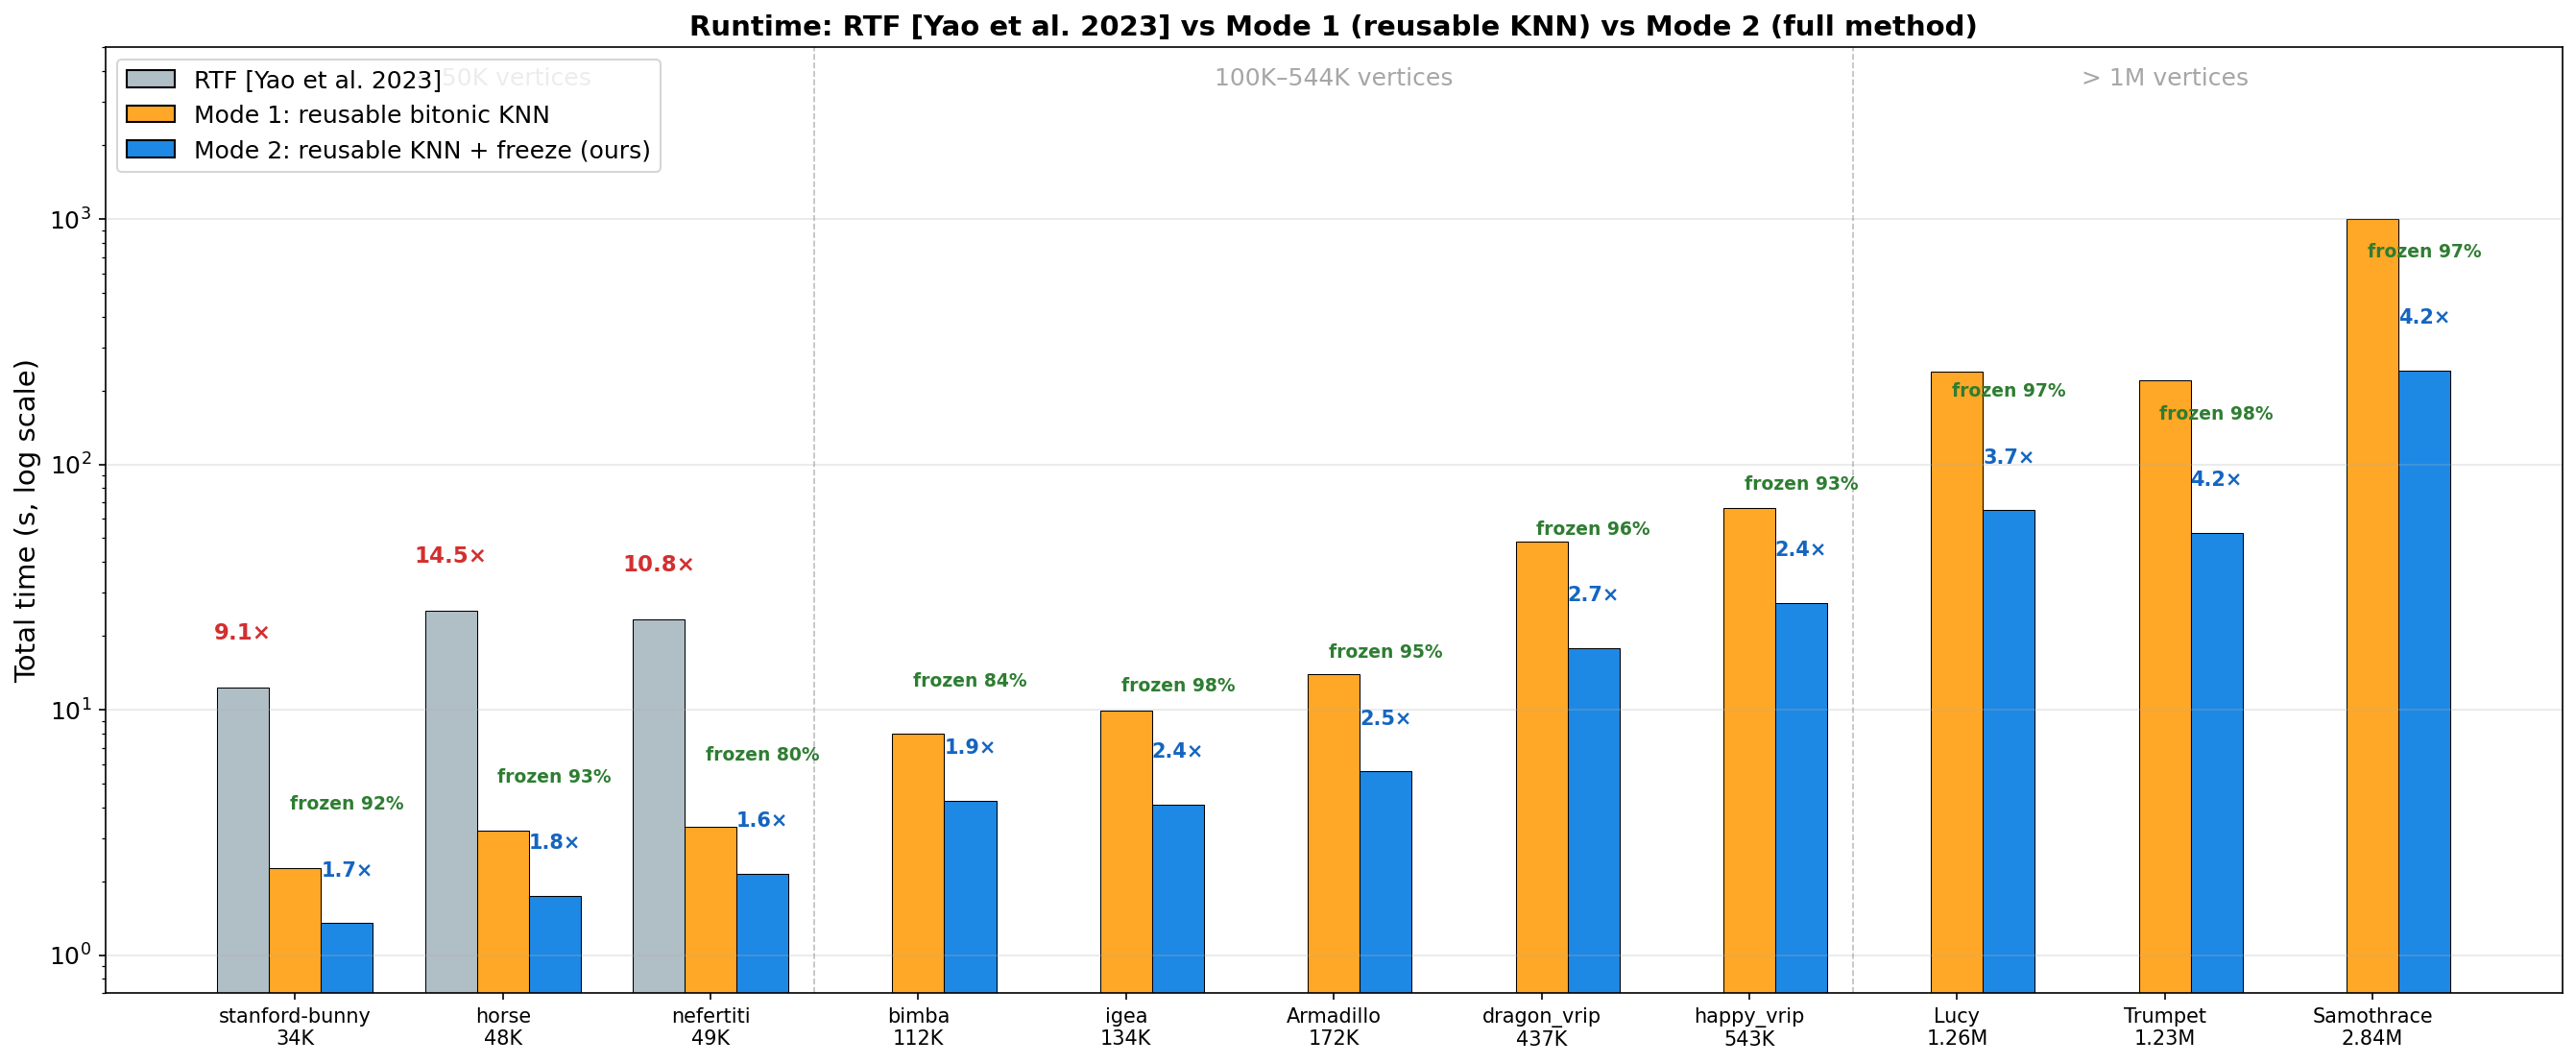
\includegraphics[width=\textwidth]{figs/fig5_speedup_bars.png}
\caption{Runtime comparison across all 11 meshes for RTF~\cite{yao2023rtf} (gray), Mode~1 (reusable bitonic KNN, orange), and Mode~2 (our full method with freeze, blue). Red annotations show RTF$\to$Mode~2 total speedup on small meshes; blue annotations show Mode~1$\to$Mode~2 freeze-only speedup; green labels indicate final freeze rates. RTF is prohibitively expensive beyond 50K vertices. The freeze advantage grows with mesh size: 1.6--1.8$\times$ at small scale, 1.9--2.7$\times$ at medium scale, and 3.7--4.2$\times$ at million-vertex scale.}
\label{fig:speedup_bars}
\end{figure*}

\subsection{Scalability}
\label{sec:scalability}

The central result of our evaluation is that the freeze advantage grows consistently with mesh size (\Cref{fig:speedup_bars}). The Mode~1 $\to$ Mode~2 speedup increases from 1.6--1.8$\times$ at 35--50K vertices, through 1.9--2.7$\times$ at 112--544K, to 3.7--4.2$\times$ at 1.2--2.8M. This trend is driven by a simple geometric argument: at higher sampling density, flat regions of the surface---which dominate most meshes---are represented by proportionally more sites. These flat-region sites converge rapidly and pass the freeze test early, while the fraction of sites near sharp features shrinks relative to the total count. The result is that the freeze rate grows from 80--93\% at small scale to over 97\% at million-vertex scale.

The practical consequences are significant. On the Samothrace mesh (2.84M vertices), Mode~1 without freezing takes 16.7 minutes. Mode~2 with freeze completes the same 250 iterations in 4.0 minutes---a 4.2$\times$ reduction. On Trumpet (1.23M), Mode~2 reduces 3.7 minutes to 53 seconds. Without the freeze policy, GPU-based CVT at million-vertex scale is impractical for iterative design workflows; with it, the runtime falls within a range that permits interactive exploration of remeshing parameters.

The effective per-iteration complexity of Mode~2 is $O((1 - f) \cdot n \cdot K)$, where $f$ is the frozen fraction. As $f$ grows toward 1 with increasing $n$, the active query count $(1 - f) \cdot n$ grows sublinearly in $n$---at 97\% frozen, only 3\% of sites are queried per iteration. This freeze-driven sublinear scaling is the mechanism through which our method extends KNN-based GPU CVT to scales where prior methods are impractical, and through which it maintains a consistent advantage over CPU Delaunay methods whose per-iteration cost scales as $O(n \log n)$ with no convergence-aware reduction.
